\documentclass[tikz,border=10pt]{standalone}
\begin{document}
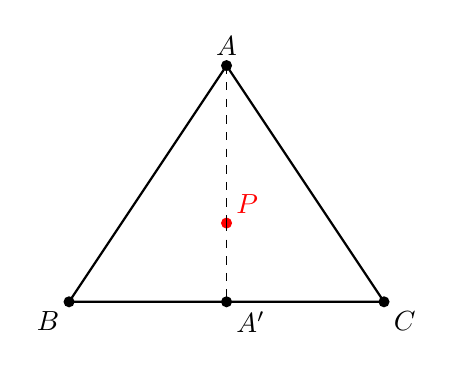
\begin{tikzpicture}

    % Define the points
    \coordinate (A) at (0, 3);
    \coordinate (B) at (-2, 0);
    \coordinate (C) at (2, 0);
    \coordinate (P) at (0, 1);
    \coordinate (Adash) at (0,0);

    % Draw the triangle ABC
    \draw[thick] (A) -- (B) -- (C) -- cycle;

    % Draw the point P
    \fill[red] (P) circle (2pt) node[above right] {$P$};

    % Draw the extended line AP
    \draw[dashed] (A) -- (P);
    
    % Extend AP to intersect BC
    \draw[dashed] (P) -- (Adash);
    

    % Label the vertices
    \fill[black] (A) circle (2pt) node[above] {$A$};
    \fill[black] (B) circle (2pt) node[below left] {$B$};
    \fill[black] (C) circle (2pt) node[below right] {$C$};
    \fill[black] (Adash) circle (2pt) node[below right] {$A'$};

    % Draw the line BC
    \draw[thick] (B) -- (C);

\end{tikzpicture}
\end{document}
